\documentclass[a4paper,12pt]{article}
\usepackage{amsmath}
\usepackage{hyperref}
\usepackage{graphicx}
\graphicspath{ {img/} }


\hypersetup{
	urlcolor=red,
	linkcolor=red,
	colorlinks=red,
}

\begin{document}
\title{Implementation of a Fuzzy Rule-Based Classifier using Genetic Algorithms}
\author{Mona Rashed,Quentin David,Joseph Yaconelli}
\date{December 2017}
\maketitle
%\pagestyle{headings}


\section{Foreword}

Our code can be download in this github link:
\url{https://github.com/Apoptoz/FL_Classifier}
To launch the program, simply type \textit{python3 GAA.py} in a terminal.
You can tune the parameters in the file GAA.py and classifier.py.\\
\\
We shared the work this way:\\
Rashed: \\
Joseph: \\
Quentin: \\

\section{Introduction}

Usually, fuzzy systems are designed by an expert. We rely on the expert to find the membership values and the rules to design the Knowledge Base.
However, there are cases where the expert is not trustworthy, there is no expert available, or a human is not able to be an expert in the problem domain. Thus, this paper is trying to explore the use of a computer heuristic, namely a Genetic Algorithm (GA), to design one part of a fuzzy rule-based classifier.

GAs are proven to be good on optimization problems. They can search through complex spaces efficiently. Moreover, the fitness function lets us implement some biases or preferences.

The goal of this project is to implement a rule based classification system using both a genetic algorithm and fuzzy logic.
We expect our algorithm to find a rule set that satisfies two objectives : accuracy \& simplicity.
We want a rule set that correctly classifies our dataset, but also has simple and human-interpretable rules.

This work is inspired by the classifier presented by Xiong, N., and Lothar Litz. in \textit{“Generating Linguistic Fuzzy Rules for Pattern Classification with Genetic Algorithms.”} (1999) based on the Iris dataset. This dataset is a well known classification dataset with four attributes and 3 classes. The attributes are Sepal Length, Sepal Width, Petal Length and Petal Width, and the classes are Iris Setosa, Iris Verticolor and Iris Virginica. \\

\section{Fuzzy Logic}

Fuzzy Logic is a theory to deal with uncertainty.
Zadeh introduced fuzzy set theory in 1965. Usually logic is seen with a Boolean approach. Is a whale a fish? Yes or no, there is no in between. This is what we call a \textit{crisp set}. Either it belongs to the set, or it's a nonmember. 
However, fuzzy sets are made to encompass the sometimes uncertain nature of an assertion. An object will belong to a fuzzy set with a certain truth value which is called the \textit{grade of membership}.
Fuzzy Logic have been applied in a lot of domains, notably in control systems and in artificial intelligence.

\begin{center}
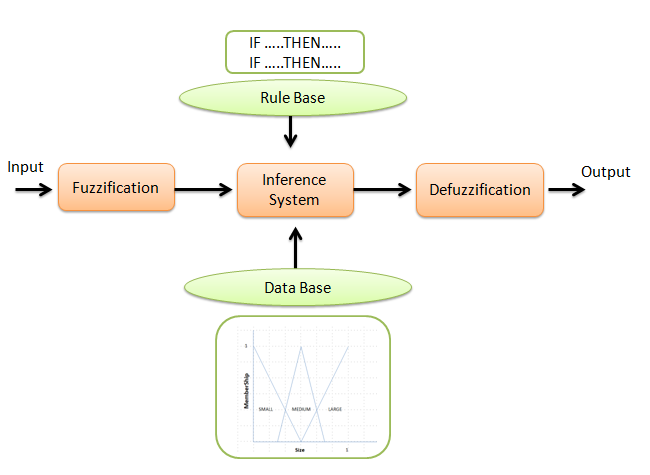
\includegraphics[scale=0.5]{fuzzysystem}
\end{center}

Fuzzification is the first step of a fuzzy system. It takes crisp input values and turns them into fuzzy values through a membership functions.
For our classifier, we have designed 3 linguistic variables for each of the parameters. In total, we have 12 membership functions.
The three linguistics variables are SMALL, MEDIUM and LARGE. We decided to have the same functions for each of the parameters.
All the parameters are normalized so we get for all a value between 0 and 1.

\begin{center}
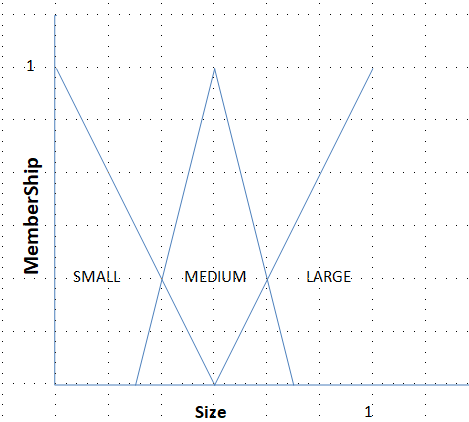
\includegraphics[scale=0.5]{fuzzymembership}
\end{center}

The inference is the process of getting an ouput given an output. For a classification task, the output will be the predicted class.
This process is described in the Fitness function section.

Finally, the defuzzification is the part where we map our output into a quantifiable crisp value. For a classification task, the defuzzification consist in taking the class with have the most average accuracy. Again, this step is explained in the fitness function section.

\section{Confidence degree of a rule}
For each of these attributes $x_{i}(i=1\cdots n)$ there are three fuzzy sets that are denoted A(i,S), A(i,M), A(i,L), respectively for Small, Medium and Large.
Let's define \textbf{p} as the mapping function from $\{1\cdots s(s\leq4)\}$ to $\{1\cdots4\}$, with $\forall x\neq y, p(x)\neq p(y)$. We use this function to express that not all parameters are needed in a rule.
Thus we can generalize rules as follows :

\[if \left( [x_{p(1)}=\bigcup_{j\in D(1)}A(p(1),j) ] \bigcap\cdots\bigcap[x_{p(s)}=\bigcup_{j\in D(s)}A(p(s),j) ] \right) then\quad \bf B \] 

With $D(i)\subseteq\{Small,Medium,Large\}$ \\
$\bigcup$ corresponds to \textbf{or} and $\bigcap$ to \textbf{and}.\\
So for example, if:
\[D(1)=\{Small\},D(2)=\{Medium,Big\},D(3)=\{\},D(4)=\{Small,Medium,Big\}\]
Then our rule would read as:
\begin{center}If Sepal Length is Small AND Sepal Width is Medium OR Big AND Petal Width is Small OR Medium OR Big, then $C_i$.\end{center} 
There are 12 different membership functions that can each be present or not in a rule. If all the functions are absent from the rule, we have an empty fuzzy set for the condition part, which is an invalid rule.\\
Thus there are $2^{12}-1=4095$ possible rules. The number of rules is exponentially increasing with the number of parameters and linguistic variables. We could have encoded the resulting class in our rules, but it would have increased the search space. \\ 
\\
Xiong \& Litz proposed a way to compute the classes using the antecedent and the data set: \\
\\
A rule can be summarised as \textit{If A then B, or $A\Rightarrow B$}.\\
$B\in \{Class_1,Class_2,Class_3,Class_4\}$\\
\[A=[x_{p(1)}=\bigcup_{j\in D(1)}A(p(1),j) ] \bigcap\cdots\bigcap[x_{p(s)}=\bigcup_{j\in D(s)}A(p(s),j)]\]
$\mu_A(u_i)$ is the membership value of an item $u_i(i=1\cdots m)$ from the training set $U_t=\{u_1,\cdots ,u_m\}$ to A.
%This time B is not C1 or C2.... Should we change ?
The consequent B is a crisp subset which is defined as follows:
\[\mu_B(u_i)=
\begin{cases}
	1 & \text{if $class(u_i)=B$}\\
	0 & \text{otherwise}
\end{cases}\]
(For the class prediction later, B will be a fuzzy subset)\\
\\
$A\Rightarrow B$ is equivalent to $A\subseteq B$, so the subsethood of A in B will be used to compute the truth value of a rule for each class:
\[
	truth(A\Rightarrow B)=
	\frac{M(A\cap B)}{M(A)}=
	\frac
		{\sum\limits_{u_i\in U_T}{(\mu_A(u_i)\land \mu_B(u_i))}}
		{\sum\limits_{u_i\in U_T}{\mu_A(u_i)}}=
	\frac
		{\sum\limits_{class(u_i)=B}{\mu_A(u_i)}}
		{\sum\limits_{u_i\in U_T}{\mu_A(u_i)}}
\]

\section{Rule Based Genetic Algorithm}

\subsection{Presentation}

Genetic Algorithm is a heuristic search algorithm based on the law of evolution to reach for an optimal solution within a problem space. GA are good for multi-dimensional problems.

\begin{center}
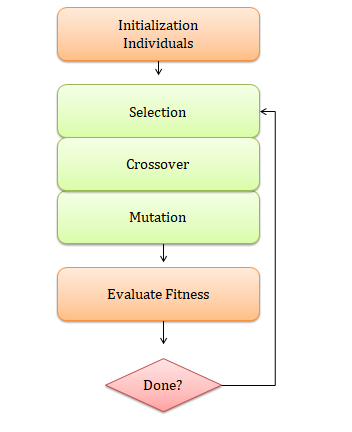
\includegraphics[scale=0.5]{genealgo}
\end{center}

There are two types of GA rule based classifiers: the Pittsburgh approach and the Michigan approach. Pittsburgh: Each chromosome is a rule set. Michigan: each chromosome is a rule, and the system evolves as a whole. We decided to use the Pittsburgh approach as it was more intuitive for us to build.


Genetic Algorithms can be used for various parts of a fuzzy system:\\
\\
Tuning the membership function\\
Rule learning\\
Rule selection\\
Learning of Knowledge Base\\
Inference parameters\\
Etc... (see \url{http://sci2s.ugr.es/sites/default/files/files/TematicWebSites/GeneticFuzzySystems/FUZZ-IEEE09_Tutorial_EMOFRBSs-Ishibuchi-Alcala.pdf})

\begin{center}
Genetic algorithm to learn a fuzzy rulebase
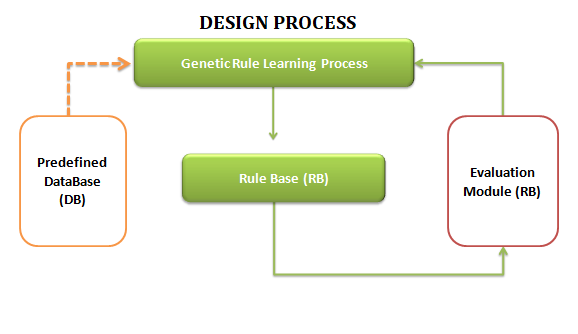
\includegraphics[scale=0.5]{genefuzzy}
\end{center}


\subsection{Modeling the algorithm}

\subsubsection{Individual}

We define an individual as a list of rules. Rules are represented with a list of 12 bits, 3 bits for each parameter.
These 3 bits express the presence or not of each linguistic variable for D(i): 1 if present, 0 otherwise.
For example, the rule presented in section 2 would be represented as [1,0,0,0,1,1,0,0,0,1,1,1].
We decided to set 10 rules for each individual.

\subsubsection{Selection and Crossover of individuals}

In genetic algorithms, it's important to avoid a \textbf{premature convergence}, that is when a population converge toward a local extremum rather than the global optimum. \\
The Tournament Selection is a way to chose a user-selected number of random individuals in a population, and then take the fittest.\\
It is possible to give a chance to weaker individuals by reducing the number of participating candidates, or in the opposite to prevent weaker ones from breed by increasing the number.
Two selections give two individuals that can mate with a crossover.
The idea is to mix the chromosomes of the individuals to produce a child inheriting the genes of his parents.\\
Many techniques exist to cross two chromosomes. We chose to pick the uniform crossover.\\
Given two rules, for each bit there is a 0.5 probability of inheriting the gene of one of the parent.\\
We repeat the process for each pair of rules.

\subsubsection{Mutation}

Mutation is a key point in letting genetic algorithms explore the problem space by maintaining a problem diversity. Similar to biological mutation, this operator modifies a chromosome in a unpredictable way and can give a better solution.
In our algorithm, there is a mutation parameter that will give the chance of each gene flipping its bit. Each bit of each rule of an individual will have a probability $p_{mut}$ of being flipped.\\
If $p_{mut}$ is too high, the information given by the chromosome might be lost because it changed too much, and thus the algorithm may never converge. However, if $p_{mut}$ is too low, the exploration space may be restricted and thus the algorithm may converge to a local optimum.

\section{Compute the fitness function}

The calculation of the fitness function is the core of our implementation.\\
We will explain in depth the structure of that function.

\begin{center}
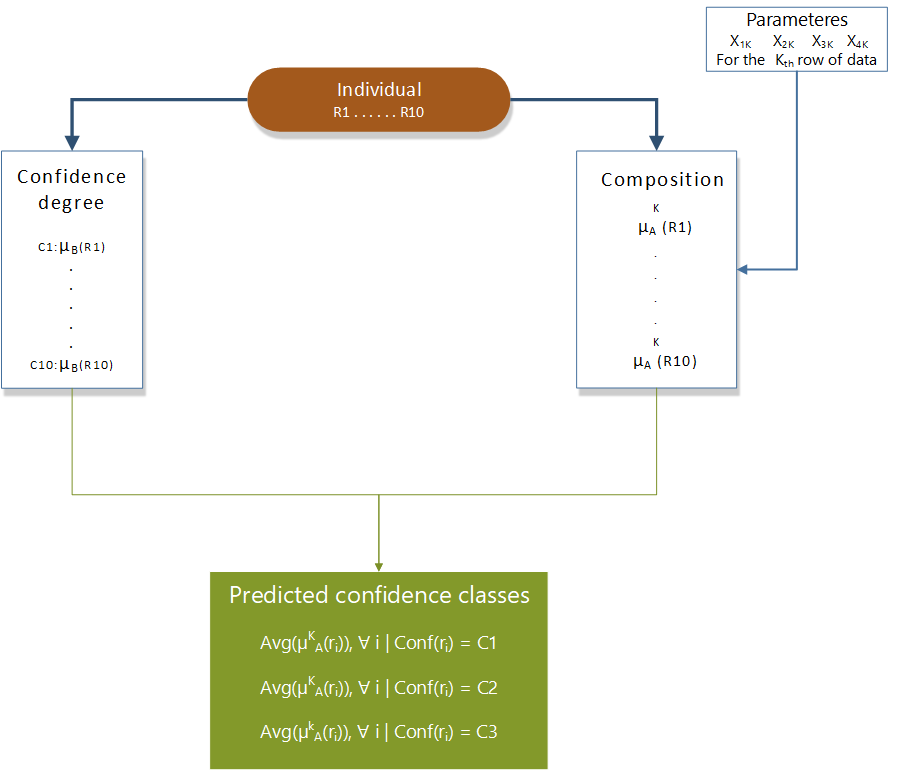
\includegraphics[scale=0.3]{fitnessfunct}
\end{center}

\subsection{Vector of best class confidence}

Given a rule, we measure the truth degree of that rule using the formula previously described on our training data for each class.
The function \textit{getConf} gives the vector :

\[
\begin{bmatrix}
C_1:\mu_b^1(r)\\
C_2:\mu_b^2(r)\\
C_3:\mu_b^3(r)
\end{bmatrix} \]

with $C_i$ the class and $\mu_b^i(r)$ the truth degree of that rule $r$ on class $i$.
\\
\\
An Individual is composed of a set of rules, so the function \textit{getConfVect} gives the vector :
\[
\vec{Conf}=
\begin{bmatrix}
C_i^1:\mu_b^i(r_1)\\
C_i^2:\mu_b^i(r_2)\\
\vdots\\
C_i^m:\mu_b^i(r_m)\\
\end{bmatrix} \]
With $m$ the number of rules. For each rule, we take the maximum $\mu_b$ from \textit{getConf}. This vector represents for each rule of an individual, what class it fits best, and with what confidence.

\subsection{Vector of $\mu_A$, given a data instance and rules}

The next step is to do fuzzy composition on each of the rules, given an instance of data, here $[x_1,x_2,x_3,x_4]$.

The function \textit{getMuA} takes two parameters: a data instance and a rule.

Remembering this formula:
\[A=[x_{p(1)}=\bigcup_{j\in D(1)}A(p(1),j) ] \bigcap\cdots\bigcap[x_{p(s)}=\bigcup_{j\in D(s)}A(p(s),j)]\]

We chose to measure $\mu_a$ like this:

\[\mu_A=
min
\begin{pmatrix}
max(A(p(1),j),\forall j \in D(1))\\
\vdots \\
max(A(p(s),j),\forall j \in D(s))
\end{pmatrix}
    \]
\textbf{Example:}\\
\\
Lets take our example rule:
\begin{center}
If Sepal Length is Small AND Sepal Width is Medium OR Big AND Petal Width is Small OR Medium OR Big
\end{center}
And a data instance (normalized): $x_1=0.97,x_2=0.86,x_3=0.97,x_4=0.88$.\\
\[
\begin{split}
\mu_A &= min
\begin{pmatrix}
max(\mu_S(0.97))\\
max(\mu_M(0.86),\mu_B(0.86))\\
max(\mu_S(0.88),\mu_M(0.88),\mu_B(0.88))
\end{pmatrix}\\
&= min
\begin{pmatrix}
max(0)\\
max(0.28,0.72)\\
max(0,0.24,0.76)
\end{pmatrix}\\
&= min(0,0.72,0.76) = 0
\end{split}
\]
\\

In the same fashion as we did for our confidence vector, we use the function \textit{getMuVect}:

\[
\vec{\mu_A^k}=
\begin{pmatrix}
\mu_A^k(r_1)\\
\vdots\\
\mu_A^k(r_m)
\end{pmatrix}
\]
For the k-th piece of data from the test data.

\subsection{Assembling the pieces: predicting a class}

We now want to get the predicted confidence of classes for an instance.\\
$\vec{Conf}$ gives us the fittest class for each rule, and $\vec{\mu_A}$ its confidence given an instance of data.
\[
\text{Predicted Classes Confidence: }
\begin{pmatrix}
avg(\mu_A^k(r_i)), \forall & i & | & Conf(r_i)=C_1\\
avg(\mu_A^k(r_i)), \forall & i & | & Conf(r_i)=C_2\\
avg(\mu_A^k(r_i)), \forall & i & | & Conf(r_i)=C_3
\end{pmatrix}
\]
Here, the class predicted will simply be the maximum average.


\subsection{Accuracy \& Fitness function}

The accuracy gives us the percentage of well predicted instances of our classification on a test data. We can use only this score as a fitness function.
However, the accuracy score is not our only concern : we would like to have the fewest rules as possible, as we want to produce a clear and simple rule system if one exists. So we have to compute a fitness function combining both the accuracy score and the complexity of the rule set.
This is where we decided to change our fitness function in this way:

\[f_{fitness}=\alpha (Accuracy)+\beta(Simplicity)\]

$\alpha$ and $\beta$ are the weights we can adjust to ask for more accuracy, or for more \textit{Simplicity}.
The \textit{Simplicity} is simply measured as one minus the sum of the number of fuzzy sets involved for all the rules of an individual divided by the maximum number of fuzzy sets. 
For example, if we have two rules :
\begin{center}[1,0,0,1,1,0,1,1,1,0,0,0] and [0,0,1,0,1,0,0,0,1,1,1,0]
\end{center}
Then the \textit{Simplicity} would be $1 - \frac{11}{24} \approx 0.54	$


\section{Results}

Our genetic algorithm proved to do exceedingly well at developing a set of rules that balanced both accuracy and simplicity. As part of refining our system, we looked at the performance as the number of rules per individual increased. We found in the end that using four or more rules gave a system that could predict our test data with an accuracy of ~95\% or better.
\begin{center}
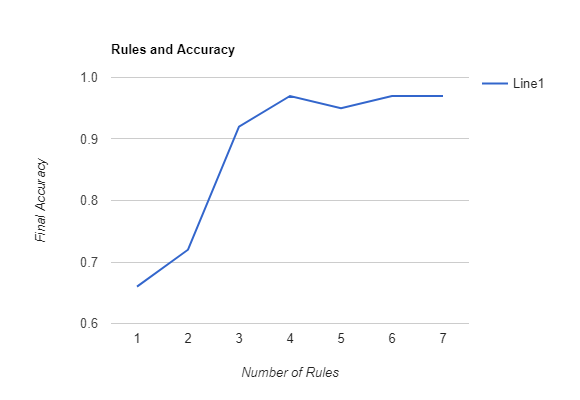
\includegraphics[scale=0.5]{accresult}
\end{center}
However, we are not only interested in getting accurate results, we also wanted to have rules that are simple and more human interpretable.
\begin{center}
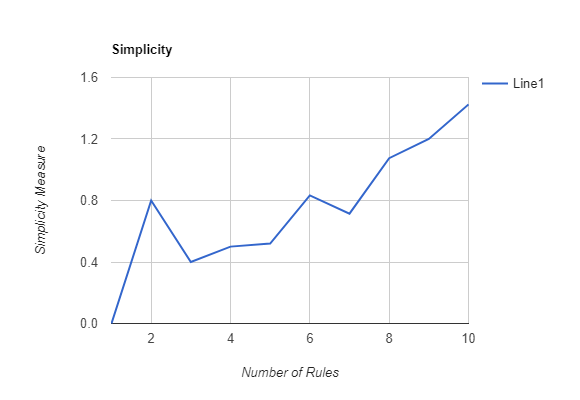
\includegraphics[scale=0.5]{simresult.jpg}
\end{center}
As shown in the above graph, as the number of rules increase the simplicity of each rule also increases. These two graphs together show the competency of our system to develop accurate and simple rules while also justifying our final choice of 10 rules because it has a high accuracy and high simplicity.
\section{Conclusion}

Based on the work of Xiong and Litz primarily, but also a lot on the work of Ishibuchi, we implemented a genetic fuzzy classifier on a basic classification task which is the Iris dataset.
We wanted to investigate how well this kind of classifier can do. Furthermore, fuzzy systems usually rely on expert knowledge. This project is also an experimentation to see if a heuristic algorithm can "find" by himself a part of the knowledge base of a fuzzy system.

There are a lot of ways to implement genetic algorithms to a fuzzy system. Here, we simply used the genetic algorithm to develop the best rule sets, with two points in mind: accuracy and simplicity.
By generating and evolving a population of rule sets, we can see convergences toward good solutions, which both have simple rules and a good accuracy, as we showed in the previous section.

In this view, we proved that a fuzzy genetic algorithm is a good classifier, and gives human-interpretable rules that other classifiers cannot give. Bayesian classifier, KNN or SVM become difficult to understand when the solution dimension is too high.
Decision tree classifier is a similar classifier to ours, but uses crisp logic. It reveals to be less efficient than our algorithm, but the rules are clear to follow.

The fuzzy genetic system however was much slower than expected. One generation takes around 20 seconds to evolve. We tried to cache the computation of the algorithm to gain more speed, but the result is not good. Furthermore, the dataset we're working on is a fairly small one, as it's composed of only 150 samples, each with 4 attributes. Our algorithm will take exponentially more time with bigger datasets, and with more features. We then doubt that this can be an effective way to classify, except if we have a lot of computation power and a real need to produce human-interpretable rules, which can be a reason as the latest AI algorithms become more and more obscure (black-box effect).

We have had other ideas to add to our program, that we sadly did not have time for.
We wanted to implement a function to create a matlab fuzzy system file, this way we can work in matlab on the knowledge base created by our algorithm.
Secondly, the confidence level gives us a value for each of the class, we have thought to include that to predict all the classes for a given individual. It would be then a Mamdani system, with the confidence of each of the classes as an output.
Lastly, as did Xiong and Litz, we wanted to implement the membership functions into our individuals, and see if it improves the accuracy. It seems quite easy to do it, as we just add 12 numbers into the gene that will match the peak of each membership functions.

 
\bibliography{GFL.bib}
\bibliographystyle{unsrt}
\nocite{*}
\end{document}